\documentclass[3p]{article}
\usepackage[T1]{fontenc}
\usepackage[utf8]{inputenc}
\usepackage{amsmath}
\usepackage{fixmath}
\usepackage{amssymb}
\usepackage{graphics}
\usepackage{breqn}
\usepackage{algorithmicx}
\usepackage[ruled]{algorithm}
\usepackage[noend]{algpseudocode}
\usepackage{titlesec}
\usepackage{graphicx}
\usepackage{subfigure}
\usepackage{tabto}
\usepackage{hyperref}
\hypersetup{
    colorlinks=true,
    linkcolor=blue,
    filecolor=blue,      
    urlcolor=blue,
    citecolor=blue,
}

\begin{document}

\title { POD-XIgA: A 1D Numerical Example}
\author{Massimo Carraturo}

\maketitle

%%%%%%%%%%%%%%%%%%%%%%%%%%%%%%%%%%%%%%%%%%%%%%%%%%%%%%%%%%%%%%%%%%%%%%%%%%%%%%%%%%%%%%%%%%%%%%%%%%%%%%%%%%%%%%%%%%%
% INTRODUCTION

\section*{Introduction}
Additive manufacturing processes (AM) or layered manufacturing (LF) or solid free form (SFF) manufacturing processes are gaining an increasing importance in many engineering fields, from mechanical to civil engineering applications. In particular in the recent years the 3D printing technology has known an exponential growth and it has been applied to produce a wide range of products. Selective laser melting (SLM) is a specific AM process where a layer of metal material powder is locally melted by means of a laser heat source. This technology presents many challenges due to the characteristics of the underlying physical problem, which presents:
\begin{itemize}
\item  high gradient of the temperature around the heat affected zone (HAZ),
\item  different size scale have to be considered for the process domain and the HAZ,
\item  three different phases of the material are involved: powder, liquid and solid,
\item  problem parameters have non-linear dependencies on the temperature field. 
\end{itemize}
Classical finite element methods (FEM) cannot efficiently deal with these kind of problem, it calls for more sophisticated simulation technologies. In the present work the application of Reduced Order Model (ROM) \cite{Rozza2009, Hesthaven_2016} to SLM processes is investigated. \par In the literature ROM-based method have been already successfully applied for heat transfer problems \cite{brands_2016, Rozza2_2009}. This numerical technique allows to speed-up the overall computational time, when several evaluation of the same problem has to be computed varying one or more parameters. There are no restrictions on the nature of the parameters which can be varied, they can include: the laser power, the laser beam size as well as the boundary conditions at different positions along the laser path.
In the literature the ROM was already applied to heat transfer problems by means of different techniques:
\begin{enumerate}
\item Classical Model Reduction: The full order model (FOM) is first solved for a small number of different parameter values (training-phase). From the set of FOM solutions (the so called \textit{snapshots}) a reduction operator is constructed using the proper orthogonal decomposition (POD). The analysis is then performed on the reduced model, which is obtained simply projecting the discrete system onto the reduced space by means of the reduction operator (ROM-phase) \cite{Michopoulos2014a}.
The main drawback of this method is that computational speed-up affect only the time required to solve the system, while the integration of the linear system still has to be performed on the full model.
\item {POD-GFEM} \cite{Aquino2008}: In this method the POD modes extracted from the set of snapshots are used to enriched the FEM basis via partition of unity \cite{Babuska1997} approach (GFEM/XFEM). The POD-GFEM allows to integrate and solve the problem on a coarse mesh enriched using POD modes. With this method high accuracy can be achived with a relatively small number of DOFs.
\item {V-GFEM} \cite{Canales2016a}: The \textit{Vademecum}-GFEM uses a different decomposition method, the so called proper generalized decomposition (PGD). This method exploits the local nature of the thermal problem. In fact, it allows to generate the solution snapshots for the PGD on a local domain by means of an eulerian reference frame. The PGD results are then used to enrich the FEM basis following the GFEM approach. The two main advantages of this method compared with the other are the reduced number of additional DOFs and the local/global feature of the method itself, since the \textit{Vademecum} is generated separately on a local domain only the nodes around the HAZ need to be enriched.
\end{enumerate}
One main objective of the present work is to integrate training and ROM-phase evaluating at the same time local enrichment functions and global solutions. To achieve such a result reduced basis method technologies are combined together with isogeometric analysis \cite{cottrell_isogeometric_2009, nguyen_isogeometric_2013} via the partition of unity method \cite{Babuska1997}.
\par
The present report is organized as follow: firstly, the numerical method is introduced and its implementational aspects are discussed. Secondly, a numerical benchmark is presented, showing the behavior of the method for a simple, one-dimensional application.

%%%%%%%%%%%%%%%%%%%%%%%%%%%%%%%%%%%%%%%%%%%%%%%%%%%%%%%%%%%%%%%%%%%%%%%%%%%%%%%%%%%%%%%%%%%%%%%%%%%%%%%%%%%%%%%%%%%
% X-PODFEM

\section*{POD based XIgA (POD-XIgA)}

In the present work we seek for a method which first allows to capture with a relatively low number of DOFs the non-linear behaviour of an AM process and secondly leads to a considerable computational speed-up. Another objective is to avoid the separation of the training and the ROM-phase. POD-XIgA approach exploits the local/global feature required in SLM applications allowing at the same time to take advantage from the higher approximation property of Isogeometric analysis (IgA).

%%%%%%%%%%%%%%%%%%%%%%%%%%%%%%%%%%%%%%%%%%%%%%%%%%%%%%%%%%%%%%%%%%%%%%%%%%%%%%%%%%%%%%%%%%%%%%%%%%%%%%%%%%%%%%%%%%%
% POD

\subsection*{Proper Orthogonal Decomposition}
There are many different techniques which allow to generate reduced basis functions. One of the most popular is the \textit{Proper Orthogonal Decomposition} also called \textit{Karhunen-Lo{\'e}ve decomposition} or \textit{Galerkin projection}, an explore-and-compress method. The parameter space is investigated generating some randomly-distributed sample points (or \textit{snapshots}), i.e. the true solution at a given parameter value. Then the method compress the continuous parameter space into a reduced one, filtering only the information which are essential to approximate the true solution space, which are the normalized orthogonal vectors (POD-modes) corresponding to the highest energetic eigenvalues. This randomness in the snapshots generation makes the POD particularly suitable to capture the casualty associated with the time evolution of the process. The POD can be also defined as a method for constructing lower-dimensional approximation of a subspace in Hilbert space, as the \textit{Single Value Decomposition} (SVD) does in a finite-dimensional space or Euclidean space.\\Given a set of \textit{M-snapshots} 
\begin{equation}
\mathcal{M}(\mathbb{P}_{h}) = \lbrace\theta(\mu)\vert\mu \in \mathbb{P}_{h}\rbrace
\end{equation}
where $\mathbb{P}_{h} \subset \mathbb{P}$ is a discrete point-set in the parameter domain and $\theta(\mu)$ the solution vector at a give $\mu$. Let $\mathbf{T}$ being the matrix whose columns are the solution vector at each snapshot, we define the \textit{solution covariance matrix} $\mathbf{Y}$ as
\begin{equation}
\mathbf{Y} = \mathbf{T}^{T} \times \mathbf{T}.
\label{eq:covarianceMatrix}
\end{equation}
The $N_{RB}$-dimensional ( where $N_{RB} < M$ is the number of eigenvalues of $\mathbf{Y}$ higher than a given tolerance) POD-space is given by the set of orthonormal vectors $\lbrace \zeta_{i} \rbrace_{i=1}^{N_{RB}} \subset \mathbb{R}^{N_{RB}}$ which solve the minimization problem \\
\indent
\begin{equation}
\min_{\lbrace\zeta_{i}\rbrace_{i=1}^{N_{RB}}}\sum_{j=1}^{M} 
\| \mathbold{\theta}_{j}(\mu) - \sum_{i=1}^{N_{RB}}(\mathbold{\theta}_{j}^{T}(\mu)\zeta_{i})\zeta_i\|_{\mathbb{V}}^{2}
\label{eq:minPOD}
\end{equation}
where $\Vert\cdot\Vert_{\mathbb{V}}$ is the norm induced by the parametrized bilinear form (we refer to \cite{Rozza2009} for further details) for a given $\mu$
\begin{equation}
\Vert\cdot\Vert_{\mathbb{V}} = \sqrt{\mathcal{B}(\cdot, \cdot; \mu)}
\end{equation}
and with
\begin{equation}
\zeta_{i}^{T}\zeta_{j} = \delta_{ij} =
    \begin{cases}
      1 &\text{if}\quad i=j, \\
      0 &\text{if}\quad i \neq j, \\
    \end{cases}
   \quad i,j=1,...,N_{RB}.
\end{equation}
\indent Algorithm \ref{PODAlg} gives a solution for (\ref{eq:minPOD}): starting from the eigendecomposition of the snapshots covariance matrix $\mathbf{Y}$, a normalized set of column vectors $\mathbf{\bar{U}}$ is derived. It allows to transform the shape functions $\phi_{k}$ used to approximate the full order problem into a set of reduced basis $\zeta_{i}$. 
\begin{algorithm}
\caption{POD}
\begin{algorithmic}[1]
\State \textit{input}: $\Theta_{i j}(\mu) \quad M\times N $\textit{snapshots}-matrix and $\phi_{i}$ vector of FOM-basis functions.
\State \textit{output}: $\zeta_{i}$ $N_{RB}-$reduced basis functions.
\State $Y_{ik}=\Theta_{ij}(\mu)\Theta_{jk}(\mu)$ 
\State $SVD(Y_{ik})=\nu_{ik}\lambda_{kk}\nu_{ki}$
\If {$\lambda_{kk} \geq tolerance$}
\State $sort(\lambda_{kk}, \nu_{ik})$
\EndIf
\State $U_{ki}=\dfrac{1}{\sqrt{\lambda_{kk}}}\sum_{j=1}^{N_{RB}}\nu_{ij}\Theta_{ik}(\mu)$ 
\State $\bar{U}_{ki}=\dfrac{U_{ki}}{\Vert U_{ki}\Vert}$ 
\State $\zeta_{i}=\phi_{k}\bar{U}_{ki}$.
\end{algorithmic}
\label{PODAlg}
\end{algorithm}

%%%%%%%%%%%%%%%%%%%%%%%%%%%%%%%%%%%%%%%%%%%%%%%%%%%%%%%%%%%%%%%%%%%%%%%%%%%%%%%%%%%%%%%%%%%%%%%%%%%%%%%%%%%%%%%%%%%
% PARTITION OF UNITY

\subsection*{Partition of Unity Method}
The partition of unity method (PUM) \cite{Babuska1997} has been already extensively employed in the analysis of multiscale problems. Its local properties and its meshless nature make this method particularly effective to deal with problems including localized phenomena, such as crack-propagation (XFEM) \cite{Moes2002}, laminated composites (S-FEM)\cite{fish_s-version_1996} and sharp thermal gradients (GFEM$^{gl}$) \cite{Ohara2013}.
The set of POD-modes $\zeta_{i}$ can be used to enrich the initial set of shape functions $\phi_{k}$ via the partition of unity expansion 
\begin{equation}
\theta_{h}(x) = \sum_{i\in I} \phi_{i}(x)\hat{\theta}_{i} + \sum_{\alpha}\sum_{j\in I_{enr}} \phi_{j}(x)\zeta_{\alpha}a_{j\alpha}
\label{PartitionOfUnity}
\end{equation}
where $I$ is the set of all nodes of the initial (coarse) discretization, $\alpha$ is the number of POD-modes and $I_{enr}\subset I$ is the set of nodes enriched by means of POD-modes. This enrichment of standard basis can be performed only if the shape functions $\phi_{k}$ satisfies the partition of unity, i.e. $\sum_{k=1}^{n}\phi_{k}(x)=1$. 

%%%%%%%%%%%%%%%%%%%%%%%%%%%%%%%%%%%%%%%%%%%%%%%%%%%%%%%%%%%%%%%%%%%%%%%%%%%%%%%%%%%%%%%%%%%%%%%%%%%%%%%%%%%%%%%%%%%
% IgA

\subsection*{Isogeometric Analysis}
Isogeometric analysis represents a novel technique which aims to integrate Computer Aided Design(CAD) and numerical analysis. This goal is achieved employing the CAD-standard technology of Non-Uniform Rational B-spline (NURBS) \cite{Piegl1997} as set of function for the analysis. The first consequence of this approach is that complex geometries can be represented exactly. NURBS also allow to arbitrary increase the inter-element continuity, leading to a more precise representation of derivatives of the field variables. Finally, higher order Ansatz spaces generated using NURBS capture complex solution with a lower number of DOFs than standard FEM techniques.
In the present work B-splines are used as basis for the analysis. In fact, these curves are easier to deal with in numerical analysis and at the same time carry over all the key features of NURBS.
\subsubsection*{B-spline basis functions}
B-splines are curves based on parametric functions, i.e. they represent a given geometry by means of parameters. The physical (geometric) space has to be mapped onto a parametric space where the parametric function is defined. In particular, to construct a B-spline a \textit{knot vector} $\Xi=\left\lbrace\xi_{1},\xi_{2},...,\xi_{n+p+1}\right\rbrace$, where $\xi_{i} \in \mathbb{R}$ is the $i^{th} knot$, $i$ is the knot index, $p$ is the polynomial order and $n$ is the number of basis functions used to construct the curve, must be specified. The knot vector in one-dimension is a non-decreasing set of coordinates in the parameter space. Knots split the parameter space into elements, which in CAD-context are called \textit{knot-span}. Geometric boundaries in the physical space are the projection of knot lines via the B-spline mapping, this mapping can be constructed using the \textbf{Cox-de Boor recursion formula}, where B-spline basis are defined starting with piecewise constants ($p=0$):
\begin{equation}
N_{i,0}(\xi)= 
\begin{cases}
      1, & \text{if}\ \xi_{i} \leqslant \xi < \xi_{i+1} \\
      0, & \text{otherwise}.
\end{cases}
\end{equation}
For $p=1,2,3,...,$ they are defined by
\begin{equation}
N_{i,p}(\xi) = \dfrac{\xi-\xi_{i}}{\xi_{i+p}-\xi_{i}}N_{i,p-1}(\xi)+\dfrac{\xi_{i+p+1}-\xi}{\xi_{i+p+1}-\xi_{i+1}}N_{i+1,p-1}(\xi).
\end{equation}
The second key ingredient for constructing a B-spline curve are the \textbf{\textit{control points}}, vector-valued coefficients of B-spline basis. Thus, given $n$ basis $N_{i,p}$ and corresponding control points $\mathbf{B_{i}}\in\mathbb{R}$ a B-spline curve is defined by:
\begin{equation}
\mathbf{C}(\xi) = \sum_{i=1}^{n}N_{i,p}(\xi)\mathbf{B}_{i}.
\end{equation}
\subsubsection*{eXtended Isogeometric analysis (XIgA)}
Using B-spline as basis for the analysis do not affect the possibility to enrich the Ansatz space via partition of unity extension. In fact, B-spline satisfies the partition of unity, thus they can be enriched using the POD modes extracted from the training phase, as previously described. The only difference with respect to the classical XFEM enrichment is that the DOFs to be enriched are not nodal values of the mesh, but they lie at the control points, which are in general non-interpolatory. Eq. \ref{PartitionOfUnity} reads now:
\begin{equation}
\theta_{h}(x) = \sum_{i\in I} N_{i,p}(x)\hat{\theta}_{i} + \sum_{\alpha}\sum_{j\in I_{enr}} N_{j,p}(x)\zeta_{\alpha}a_{j\alpha},
\label{IgAPartitionOfUnity}
\end{equation}
which is the numerical approximation of the so-called eXtended Isogeometric analysis (XIgA) using POD-modes as enrichment functions.

%%%%%%%%%%%%%%%%%%%%%%%%%%%%%%%%%%%%%%%%%%%%%%%%%%%%%%%%%%%%%%%%%%%%%%%%%%%%%%%%%%%%%%%%%%%%%%%%%%%%%%%%%%%%%%%%%%%
% Impementation
\begin{figure}[!h]
\centering
  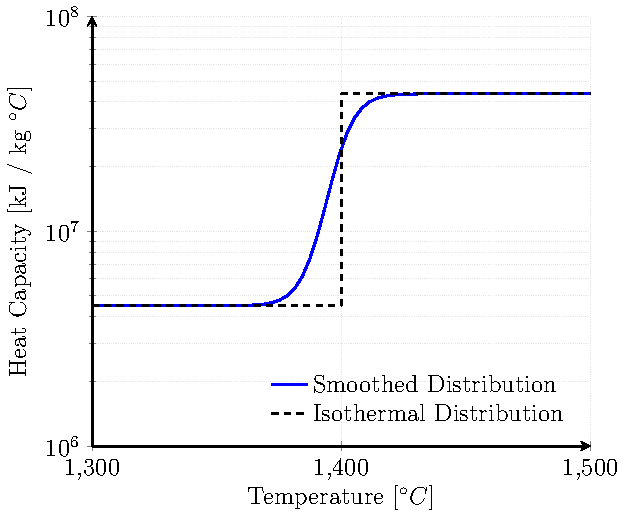
\includegraphics[width=0.5\linewidth]{externals/Pictures/heatCapacity.pdf}
  \caption{Steel heat capacity distribution}
  \label{fig:heatCapacity}
\end{figure}

\begin{figure}[h!]
\centering
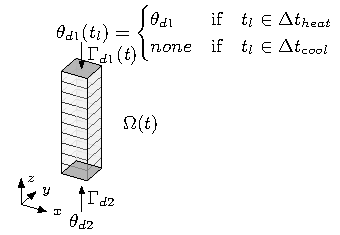
\includegraphics[width=0.8\linewidth]{externals/Pictures/PODXIGAProblemDomain.pdf}
\caption{evolution in time of the bar. The upper boundary condition depends on the layer relative time $t_{l}$. Over the total layer construction time $\Gamma_{1}$ is initially heated by means of a laser source, reaching a temperature $\theta_{d1}$. Succesively, during the powder deposition process of the next layer no heat sources are applyed anymore.}
\label{PODXIGADomain}
\end{figure}


\section*{Implementational aspects}

Following \cite{Celentano1994}, let us consider a one-dimensional thermal transient problem with phase-change in terms of volumetric enthalpy $\mathrm{H}=\mathrm{H}(\theta)$ and a domain $\Omega = \Omega(t)$ evolving in time. During an AM process 
the layer time interval $\Delta t_{l}$ can be split in two sub-intervals: $\Delta t_{h}$ when the tip of the bar is heated by means of the laser beam and reaches a temperature value of $\theta_{d1}$ and $\Delta t_{c}$ when no heat source is applied on the top of the bar. Let $\Gamma = \Gamma(t_{l})$ being a function of the layer relative time $t_{l} \in \Delta t_{l}$, at a given time $t_{l}\in \Delta t_{h}$ the problem is defined as:

\begin{equation}
\begin{cases}
    \dfrac{\partial\mathrm{H}}{\partial t}-\nabla \cdot (k\nabla\theta)=0 & \text{in}\quad \Omega \\
 	\theta = \theta_{d1} & \text{on}\quad \Gamma_{1} \\
 	\theta = \theta_{d2} & \text{on}\quad \Gamma_{2} 
\end{cases}
\label{PoissonTransientProblemHeatingPhase}
\end{equation}
while if $t_{l}\in \Delta t_{h}$, it reads:
\begin{equation}
\begin{cases}
    \dfrac{\partial\mathrm{H}}{\partial t}-\nabla \cdot (k\nabla\theta)=0 & \text{in}\quad \Omega \\
 	\theta = \theta_{d1} & \text{on}\quad \Gamma_{1} \\
 	\theta = \theta_{d2} & \text{on}\quad \Gamma_{2} 
\end{cases}
\label{PoissonTransientProblemCoolingPhase}
\end{equation}

\begin{figure}[h!]
\centering
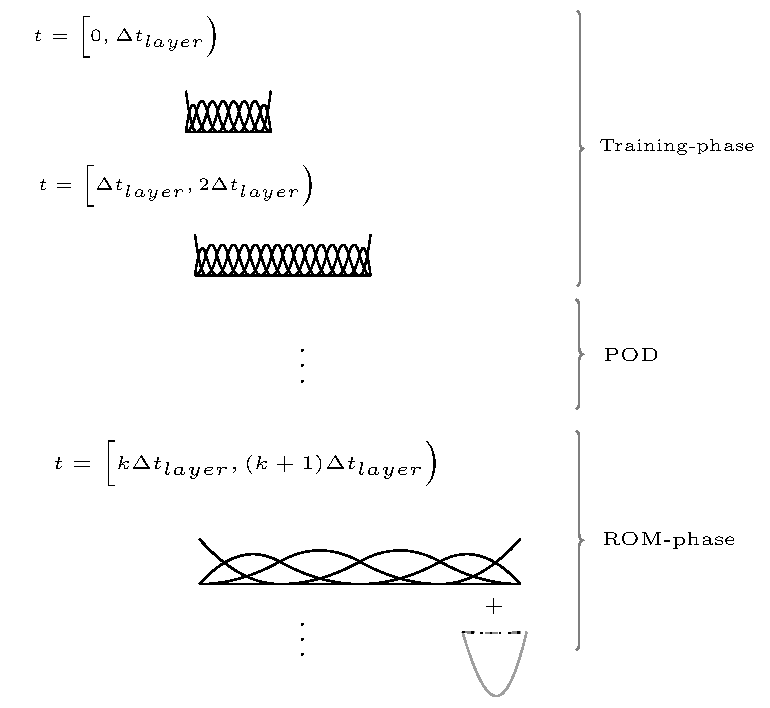
\includegraphics[width=0.8\linewidth]{externals/Pictures/PODXIGAScheme.pdf}
\caption{In the training-phase the first few layers are solved using IgA with a fine mesh and the temperature values of the last layer are recorded for a given set of evaluation points. On these temperature values POD is performed and a set of POD modes is extracted. In the ROM-phase a much coarse knot vector is considered (one knot-span/layer), the POD modes are now used to enrich the DOF associated with the last control point.}
\label{PODXIGAScheme}
\end{figure}

where the primary variable $\theta$ is the temperature, $\kappa$ is the thermal conductivity and $\theta_{d2}$ is the constant Dirichlet condition on $\Gamma_{2}$. The volumetric enthalpy is defined as
\begin{equation}
\mathrm{H}(\theta)=\int_{\theta_{0}}^{\theta}\rho c(\theta) \text{d}\theta+\rho\mathrm{L}f_{pc}(\theta),
\end{equation}
where $\rho$ is the density, $c(\theta)$ the temperature dependent specific heat capacity, $\mathrm{L}$ the latent heat, $\theta_{0}$ a reference temperature and $f_{pc}$ is the smoothed phase-change function of Figure \ref{fig:heatCapacity}.
\par
Figure \ref{PODXIGAScheme} shows as the process simulation can be split into three separate steps:
\begin{enumerate}
\item Training-phase: a FOM simulation employs a fine knot vector to solve the partial differential equations (PDE) underlying the physical problem.
\item POD: POD-modes are extracted from the set of temperature solutions registered during the training phase.
\item ROM-phase: the problem is solved on a locally enriched IgA patch.
\end{enumerate}
At each time step the temperature results on the last layer of the bar are cached for a given set of temperature evaluation points distributed around the HAZ. This approach leads to POD solutions which are mesh independent. The distribution of temperature evaluation points and mesh grid are decoupled: the temperature evaluation points are distributed relatively to the location of the laser source and do not depend on the underlying mesh. In other words a local grid is generated such that at each node of the grid the POD modes can be evaluated. \\
\indent 
Using POD-XIgA requires additional mapping for the integration of the extended term in Eq. \ref{IgAPartitionOfUnity}. From Algorithm \ref{PODAlg} we obtain a set of vectors $\zeta_{i}$ of $n$ coefficients. In order to perform numerical analysis we need an explicit function of \textbf{x}, which has to be integrated using numerical integration schemes. Therefore, the coefficients of each POD mode are interpolated using linear functions $\phi(x)$, such that
\begin{equation}
\zeta_{\alpha}^{h}(x) = \sum_{i}\phi(x)\hat{\zeta}_{i\alpha}.
\end{equation} 
The interpolation functions $\phi(x)$ are defined on a sub-domain $\bar{\Omega}$ of the integration space $\tilde{\Omega}$ (see Figure \ref{fig:IntegrationMappingPODXIgA}. An additional affine mapping $\bar{\sigma}:\bar{\Omega}^{sel}\rightarrow\tilde{\Omega}^{el}$ from the sub-domain space to the element integration space, is needed.
\begin{figure}
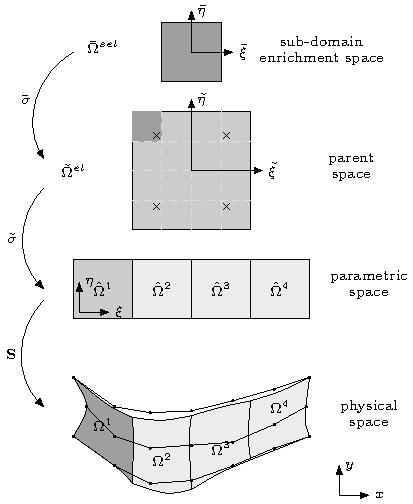
\includegraphics[width=1\linewidth]{externals/Pictures/IntegrationXPOD.pdf}
\caption{Integration is performed by gaussian quadrature on the parent space. The value of the POD-modes at each Gauss point is obtained by linear approximation of the mode coefficients. This set of coefficients define a grid, where each cell is a support for linear interpolation functions.}
\label{fig:IntegrationMappingPODXIgA}
\end{figure}
\par 
The POD-modes represents the general behaviour of the solution up to the last snapshot is recorded. When the transient problem reaches a stationary regime, i.e. the temperature distribution starts to behave always with a similar pattern, the POD-modes calculated so far allow to capture the main features of the solution using a relatively small number of DOFs. It is clear that the construction of POD-modes (training-phase), plays a vital role in this methodology.



%%%%%%%%%%%%%%%%%%%%%%%%%%%%%%%%%%%%%%%%%%%%%%%%%%%%%%%%%%%%%%%%%%%%%%%%%%%%%%%%%%%%%%%%%%%%%%%%%%%%%%%%%%%%%%%%%%%
% NUMERICAL RESULTS

\section*{1D Numerical Example}
\begin{figure}
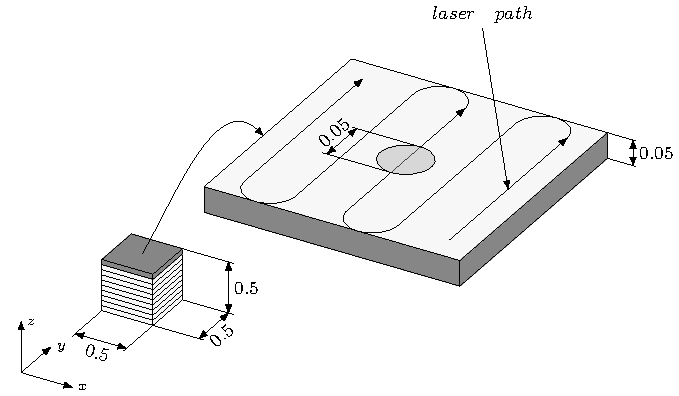
\includegraphics[width=\linewidth]{externals/Pictures/PODXIGABenchmarkBAR.pdf}
\caption{A 10 layers bar has to be constructed. Each layer is generated by a laser heat source having a radius of $0.05mm$ and moving along the laser path.}
\label{PODXIGABenchmark}
\end{figure}
As benchmark to test the method presented so far an SLM process to construct the bar of Figure \ref{PODXIGABenchmark}, is considered. The process parameters are reported in Table \ref{table::processParameters}, \ref{table::laserParameters} and \ref{table::materialParameters}. The problem is modelled using a 1D bar with a growing domain as the one discussed in the previous section.
In order to evaluate the accuracy and the efficiency of POD-XIgA, the averaged relative L2 error $err_{L2,av}\left[\%\right]$ on the last layer is computed as

\begin{equation}
err_{L2,av} = \sum_{i=1}^{10}\sqrt{\dfrac{(\theta_{ref,i}-\theta_{i})^{2}}{\theta_{ref,i}^2}}\times 100\left[\%\right],
\end{equation}

where $\theta_{ref,i}$ is the reference temperature solution vector of the $i^{th}$ time step at the last layer of the process, obtained using IgA with $2^6\times layers$ knot-spans and $\theta_{i}$ is the POD-XIgA solution at the last layer of the same time step. Figure \ref{L2DofsError} shows the convergence plot of the $err_{L2,av}$ with respect to the number of DOF. Results for the POD-XIgA method integrated using gaussian quadrature with $(n_{modes}+1)$ still presents an integration error which increases with the number of modes $n_{modes}$. In the $Overintegrated$ case, with $20\times$ more quadrature points, we observe that POD-XIgA results are considerably improved. The drawback is that the high amount of Gauss points required to exactly integrate the POD-modes using gaussian quadrature, strongly decreases the computational  efficiency of the method. Leaving the integration issue as an open task to further investigations, in Figure \ref{L2TimeError} can be observed that, even using a non-optimal quadrature rule, POD-XIgA leads to the same level of accuracy of a standard IgA patch having three more levels of hierarchical refinement (i.e. each knot-span of one level contains two knot-spans of the level below) and a computational speed up by a factor $>2$.
A good agreement with the highly refined reference IgA solution is observed also in heat flux distribution of Figure \ref{HeatFluxes}. 

\begin{table}[!h]
\centering
    \begin{tabular}{ | l | l | l | p{5cm} |}
    \hline
    number of layers & $10$\\ \hline
    total construction time & $4.5$ $sec$\\ \hline
    laser path length & $0.5$ $mm$\\  \hline
    laser time ($\Delta T_{laser}$) & $0.18$ $sec$\\  \hline
    cooling time ($\Delta T_{cooling}$) & $0.27$ $sec$\\  \hline
    total time per layer ($\Delta T_{layer}$) & $0.45$ $sec$\\  
    \hline
    \end{tabular}
\caption{Bar parameters}
\label{table::processParameters}
\end{table}

\begin{table}[!h]
\centering
    \begin{tabular}{ | l | l | l | p{5cm} |}
    \hline
    number of time steps /layer & 10\\ \hline
    laser radius & $0.05$ ${mm}$\\ \hline
    laser speed & $2.78$ ${mm}/{sec}$\\ \hline
    initial temperature & $20^{\circ}C$\\ \hline
    laser temperature & $1520^{\circ}C$\\ 
    \hline
    \end{tabular}
\caption{Layer parameters}
\label{table::laserParameters}
\end{table}

\begin{table}[!h]
\centering
    \begin{tabular}{ | l | l | l | p{5cm} |}
    \hline
    density($\rho$) & $7500 \quad {kg}/{m^{3}}$\\ \hline
    specific heat capacity($c$) & $600 \quad {J}/{kg^{\circ}C}$\\ \hline
    latent heat($\mathrm{L}$) & $2.61e^{5} \quad {J}/{kg}$\\  \hline
    thermal conductivity ($k$) & $27 \quad {W}/{m^{\circ}C}$\\ 
    \hline
    \end{tabular}
\caption{Material parameters}
\label{table::materialParameters}
\end{table}

\begin{figure}[!h]
\centering
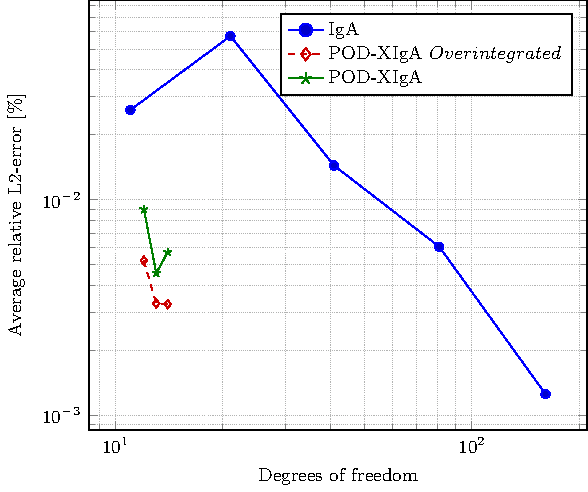
\includegraphics[width=0.75\linewidth]{externals/pgfplots/PODXIGA/L2ErrorVsDofs.pdf}

    \caption{L2 error at the last layer of the process vs degrees of freedom.}
    \label{L2DofsError}
\end{figure}

\begin{figure}[!h]
\centering
  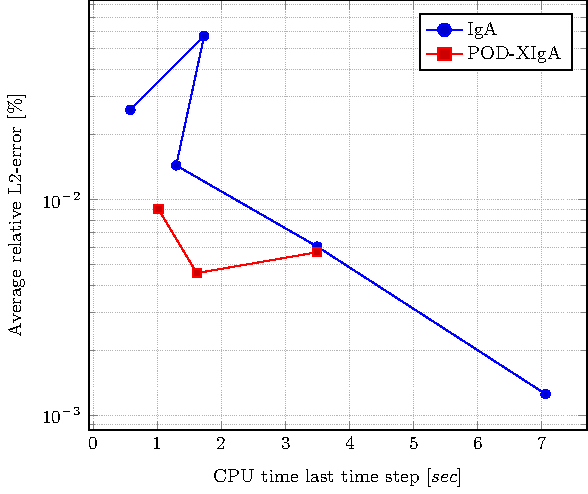
\includegraphics[width=0.75\linewidth]{externals/pgfplots/PODXIGA/L2ErrorVsCPUTime.pdf}
    \caption{L2 error at the last layer of the process vs CPU time.}
	\label{L2TimeError} 
\end{figure}

\begin{figure}[!h]
\centering

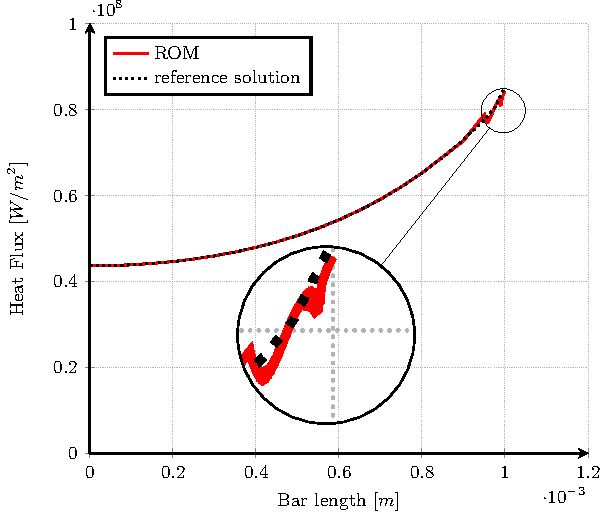
\includegraphics[width=0.75\linewidth]{externals/pgfplots/LastLayerFluxesComparisonMultiscale.pdf}

    \caption{Heat fluxes distribution along the bar after 10 layers at the $1^{st}$, $4^{th}$ and $10^{th}$ time step.}
    \label{HeatFluxes}
\end{figure}

%%%%%%%%%%%%%%%%%%%%%%%%%%%%%%%%%%%%%%%%%%%%%%%%%%%%%%%%%%%%%%%%%%%%%%%%%%%%%%%%%%%%%%%%%%%%%%%%%%%%%%%%%%%%%%%%%%%
% CONCLUSION 

\section*{Conclusion and further outlooks}


A key feature of POD-XIgA approach is that POD-modes are independent from the underlying IgA patch. This features plays a vital role if we consider that ROM-based method fails if the problem is not stationary. Therefore, if we aim to simulate a full AM process with an arbitrary complex geometry, an efficient numerical scheme is required not only for the stationary part of the problem but also for the non-stationary (training) phases. With the POD-XIgA a locally refined IgA patch can be used to both generate mesh independent POD-modes and simulate the non-stationary phases of the process. This flexibility of the method is essential to overcome the limit of general ROM-based approaches which are burden with an expensive numerical scheme for the training phase and consequently for the non-stationary part of the manufacturing process.

The method, even if tested only for a simple one-dimensional benchmark, shows results in good agreement with the reference solution. Nevertheless it presents a non-negligible integration error.
To the best knowledges of the author there are not specific integration techniques to efficiently integrate modal enriched Bspline basis functions. This issue strongly burden the effectiveness of the method. In fact, it is reasonable to expect that moving to higher dimensions, the enriched functions will required an even higher number of integration points to reach an acceptable accuracy in the integration. The possibility to gain an effective computational speed-up are thus strongly limited.

\bibliographystyle{abbrv}
\bibliography{bibliography.bib}

\end{document}

